\documentclass{ximera}



\begin{document}
        \author{Bert Lambregs}
        \xmtitle{Oefeningen (per bestand, toep.)}

\section{Newton}


\item Twee ploegen zijn aan het touwtrekken. Volgens het derde
beginsel van Newton oefenen de twee ploegen steeds even grote maar tegengestelde krachten op elkaar uit. Hoe is het dan mogelijk dat er toch een winnende ploeg is?
\begin{oplossing}
\newline
Er is een winnende ploeg mogelijk omdat het samenstellen van krachten op elke ploeg afzonderlijk gebeurt. Het zijn niet de actie- en reactiekracht (derde wet van Newton) die worden samengesteld. 

De winnende ploeg slaagt erin zich beter af te zetten dan de verliezende ploeg. Dat wil zeggen dat de reactiekracht van de kracht die ze op de grond uitoefenen (de weerstandskracht dus) groter is dan de kracht tussen de twee ploegen. De resulterende kracht van de weerstandskracht en de spankracht op de ploeg, zorgt volgens de tweede wet van Newton voor een versnelling; de ploeg komt in beweging. Voor de verliezende groep is dat net omgekeerd.  
\end{oplossing} % touwtrekken
\item Hoe komt het dat een vrachtwagen binnen een veel kortere afstand kan stoppen dan een trein die dezelfde snelheid heeft? % Inzicht 2de wet van Newton

\begin{exercise}

% !TEX root = ../main.tex


\pt{5}Je springt vanuit een roeibootje naar de oever. Verklaar wat er kan gebeuren als het roeibootje niet is vastgemeerd. Wanneer je nu vanaf een groot binnenschip naar de oever springt, wat zou het resultaat dan zijn? Verklaar!
\begin{oplossing}

Bij een roeibootje dat niet vastgemeerd is, is er veel kans dat je in het water belandt. Bij het afzetten, schiet het bootje namelijk gemakkelijk onder je weg. Hoe komt dat? Wel, doordat je je afzet, oefen je een kracht uit op het bootje. De \textbf{derde wet van Newton} zegt dat het bootje dan een even grote kracht op jou uitoefent, in de tegengestelde richting. Het is die reactiekracht die je zou willen aanwenden om op de oever te geraken. De massa van het bootje is echter zo klein in vergelijking met jouw massa dat, volgens de \textbf{tweede wet van Newton} ($\vec{F}=m\vec{a}$), de versnelling die het bootje krijgt als gevolg van jouw actiekracht veel groter is dan de versnelling die je zelf krijgt door de afzet. In de korte tijd dat je jezelf kan afzetten, verwerft het bootje dus een grote snelheid waardoor het onder je wegschiet en krijg jij geen noemenswaardige snelheid opgebouwd.

%Als het bootje is vastgemeerd, lukt het je wel de oever te bereiken. Het bootje kan immers niet wegschieten waardoor je je voldoende lang kan afzetten (er werkt voldoende lang een kracht op jou) en zo de nodige snelheid kan verwerven (je krijgt immers een versnelling) om de sprong te kunnen maken.

Voor een groot binnenschip is de massa zo groot in vergelijking met die van jou, dat het binnenschip een verwaarloosbare versnelling weg van de oever krijgt. Je kan een voldoende grote versnelling opbouwen die lang genoeg aanhoudt om je op de oever te krijgen.
\end{oplossing}



%\item Je springt vanuit een roeibootje naar de oever. Verklaar wat er kan gebeuren als het roeibootje niet of wel vastgemeerd is. Wanneer je nu vanaf een groot binnenschip naar de oever springt, wat zou het resultaat dan zijn? Verklaar!

\end{exercise}
 % Roeibootje. Inzicht 2de en 3de wet van Newton
% !TEX root = ../main.tex



\item\pt{4}\begin{minipage}[t]{.6\linewidth}
	Wat klopt er fysisch niet aan wat er gebeurt in de cartoon? Licht toe.
\end{minipage}
\hfill
\begin{minipage}[t]{.37\linewidth}
	\raisebox{6ex-\height}{%
		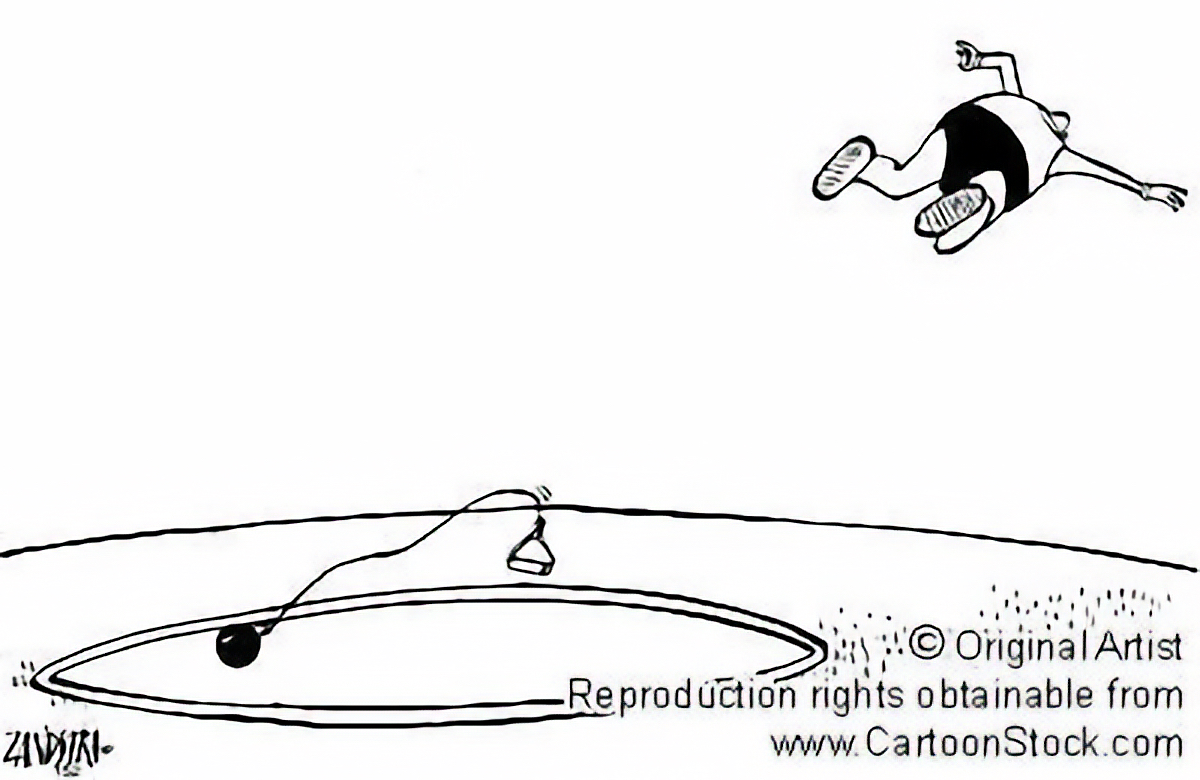
\includegraphics[width=\textwidth]{jza0018l}%
		} 
\end{minipage}


\begin{oplossing}

De hamerslingeraar wordt weggeslingerd door de kogel stil blijft liggen. Het moet omgekeerd zijn.




ChatGPT

Waarom vliegt bij het hamerslingeren de kogel weg en niet de persoon?

Bij het hamerslingeren draait alles om de centripetale kracht die op de kogel (het hamerhoofd) wordt uitgeoefend wanneer het aan een draad wordt rondgedraaid voordat het wordt losgelaten. Laten we dit proces in meer detail bekijken:

1. **Centripetale kracht:** Wanneer de atleet het hamerhoofd rondzwaait, ervaart de kogel een centripetale kracht die naar het middelpunt van de cirkel is gericht (in dit geval het draaipunt van de draad). Deze kracht zorgt ervoor dat de kogel voortdurend naar het centrum van de cirkel wordt getrokken.

2. **Inertie van de persoon:** Tegelijkertijd ervaart de atleet, die de kogel rondzwaait, een tegenovergestelde reactie volgens de derde wet van Newton: "Actie is reactie". De atleet oefent een kracht uit op de kogel, maar de kogel oefent ook een gelijke maar tegengestelde kracht uit op de atleet.

3. **Massaverschil:** Het belangrijke verschil hier is het verschil in massa tussen de atleet en de kogel. De kogel heeft veel meer massa dan de atleet. Volgens de tweede wet van Newton (F = m * a), waarbij F de kracht is, m de massa en a de versnelling, zal de kogel minder versnellen dan de atleet, omdat de kracht gelijk is maar de massa veel groter is.

Samenvattend zorgt de centripetale kracht ervoor dat de kogel in een cirkelbaan blijft, terwijl de atleet, vanwege het massaverschil, veel meer versnelt dan de kogel. Daarom blijft de kogel rondzwaaien, terwijl de atleet niet wordt weggeslingerd.

\end{oplossing} % Inzicht in de 2e en 3e wet van Newton

\begin{exercise}

% !TEX root = ../main.tex


\pt{4}Een eekhoorntje glijdt over een gladde tafel met een heleboel nootjes tussen zijn voorpoten. Wat zou hij moeten doen om te verhinderen dat hij van de tafel valt? Leg uit.

\begin{oplossing}
...
\end{oplossing}

\end{exercise}
 % Eekhoorntje en nootjes	

\begin{exercise}

% !TEX root = ../main.tex


\pt{4}Waarom gaat een boot niet vooruit als een persoon die in de boot staat krachtig tegen de wand duwt?


\begin{oplossing}
...
\end{oplossing}

\end{exercise}
 % Tegen de wand van een schip duwen.

\begin{exercise}

% !TEX root = ../main.tex


\pt{2}Kan een voorwerp bewegen zonder dat er een kracht op werkt? Leg uit.


\begin{oplossing}
...
\end{oplossing}

\end{exercise}
 % Traagheid
% !TEX root = ../main.tex


\item\pt{4}Hoe komt het dat je gemakkelijk vaststelt dat de aarde een kracht uitoefent op een appel, maar dat je niets merkt van de kracht door de appel op de aarde uitgeoefend?


\begin{oplossing}
...
\end{oplossing} % Aarde en appel

\begin{exercise}

% !TEX root = ../main.tex


\pt{3}We hebben een eenparig veranderlijke rechtlijnige beweging (EVRB) in eerste instantie binnen de kinematica behandeld. Binnen de dynamica kan je vervolgens de voorwaarden voor zo'n beweging in termen van krachten geven. 

\begin{enumerate}
\item Doe dat (wat moet er dus gelden voor de krachten om een EVRB te krijgen?), 
\item licht kort toe,
\item en geef een voorbeeld.
\end{enumerate}

\begin{oplossing}
Zie in het handboek de inleiding p. 7, de definitie van een EVRB op p. 23, de oorzaak van een versnelling op p. 29 (en eventueel ook p. 50) en de tweede wet van Newton onderaan p. 54.
\end{oplossing}

\end{exercise}
 % Dynamica EVRB

\begin{exercise}

% !TEX root = ../main.tex


\pt{3}Waarom is er in de fysica geen wetmatigheid die de wet van de traagheid verklaart net zoals we met de zwaartekracht de wetmatigheid dat lichamen in vacu\"um eenparig versneld vallen kunnen verklaren?

\begin{oplossing}
Sure! Here’s a physics test question:

Question:
Why is Newton’s First Law of Motion considered a fundamental principle in physics rather than a derivable result?

Answer:
Newton’s First Law of Motion is considered a fundamental principle because it defines the concept of inertia and establishes the framework for understanding motion in the absence of external forces. It is not derived from other laws but serves as a foundational postulate upon which classical mechanics is built. This principle highlights that an object will remain at rest or move in a straight line at constant velocity unless acted upon by an external force.

\end{oplossing}

\end{exercise}



\section{Newton Toepassingen}




\begin{exercise}

 Waarom valt in het luchtledige een massa van \SI{2}{kg} niet twee keer zo snel als een massa van \SI{1}{kg}?

\begin{oplossing}
In het vacu\"um werkt op een vrije massa enkel de zwaartekracht in. Dat is dan ook de resulterende kracht op de massa. Die kracht is inderdaad twee keer zo groot voor een twee keer zo grote massa, maar een twee keer zo grote massa verzet zich ook twee keer zo hard tegen het het veranderen van beweging; de traagheid is twee keer zo groot. Het resultaat is dat elk object met dezelfde versnelling naar de aarde valt.

Die hierboven eerder kwalitatieve redenering is kwantitatief uit te leggen met de tweede wet van Newton, $\vec{F}=m\vec{a}$:
\begin{equation*}
F_z=ma%\\
%&\Downarrow&\\
\end{equation*}
Met de formule $F_z=mg$ voor de zwaartekracht vinden we
\begin{equation*}
mg=ma%\\
%&\Downarrow&\\
\end{equation*}
Zodat, na de massa's te hebben geschrapt
\begin{equation*}
a=g%\\
%&\Downarrow&\\
\end{equation*}
De massa van het object heeft m.a.w. geen invloed op de versnelling waarmee het valt. Die versnelling is constant en in waarde gelijk aan de waarde van de veldsterkte. Omdat ook de eenheden overeenkomen (uit de tweede wet van Newton volgt dat \SI{}{N}=\SI{}{kg\cdot m/s^2}) wordt het symbool $g$ voor zowel de veldsterkte als de valversnelling gebruikt. Bij ons heeft die de waarde \SI{9,81}{m/s^2}.
\end{oplossing}

\end{exercise}
 % Valversnelling onafh. m

\begin{exercise}

% !TEX root = ../main.tex



\pt{3}\begin{minipage}[t]{.74\linewidth}
	Een massa van \SI{2,0}{kg} bevindt zich in een lift aan een dynamometer. Die laatste duidt een kracht van \SI{10}{N} aan.
\newline
%\newline	
	
	Welke beweging voert de lift uit? Licht toe.
\begin{enumerate}

	\item De lift beweegt naar omlaag met een versnelling van \SI{5,0}{m/s^2}.
	\item De lift beweegt naar omhoog met een versnelling van \SI{5,0}{m/s^2}.
	\item De lift beweegt naar omlaag met een constante snelheid.
	\item De lift beweegt naar omhoog met een constante snelheid.

\end{enumerate}
\end{minipage}
\hfill
\begin{minipage}[t]{.2\linewidth}
%\flushright
	\raisebox{1ex-\height}{%
		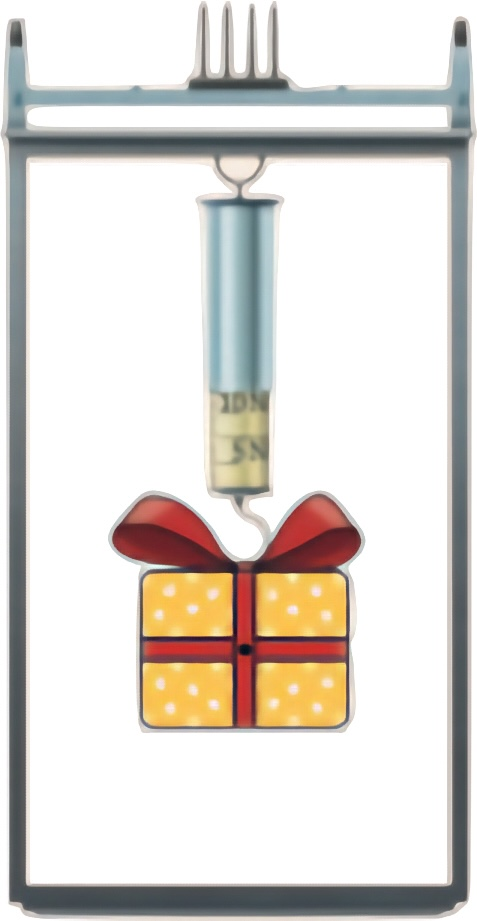
\includegraphics[width=\textwidth]{dyn/exercises/9p143}%
		} 
\end{minipage}

\end{exercise}
 % Lift en dynamometer

\begin{exercise}

 Een doos van $10\rm\,kg$ wordt met een kracht van $40\rm\,N$ over een glad tafeloppervlak getrokken. De uitgeoefende kracht maakt een hoek van $30^\circ$ met de horizontaal. Als de wrijving mag worden verwaarloosd, bepaal dan
\newline
%\begin{figure}[h]
%\begin{center}
%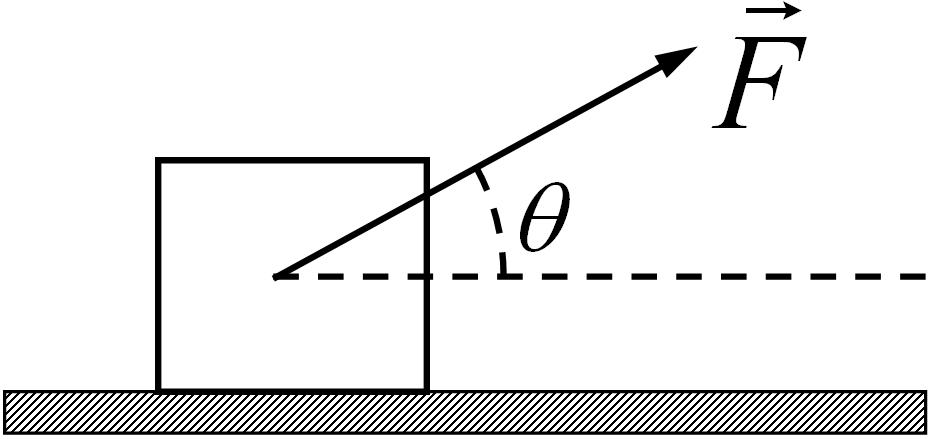
\includegraphics[width=0.4\textwidth]{dyn/exercises/doos_kracht}
%\end{center}
%\end{figure}
%\newline
%
%
\begin{minipage}[t]{.6\linewidth}
\begin{enumerate}
\item de versnelling van de doos,
\item de grootte van de normaalkracht, die de tafel op de doos uitoefent.
\end{enumerate}
\end{minipage}
\begin{minipage}[t]{.4\linewidth}
\vtop{%
  \vskip-1ex
  \hbox{%
    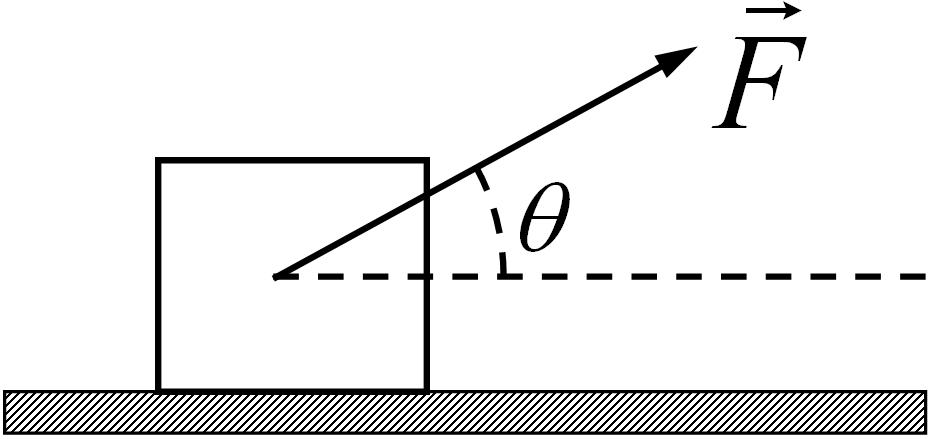
\includegraphics[width=\linewidth]{dyn/exercises/doos_kracht}%
  }%
}
\end{minipage}
%
%
%
%Als de wrijving mag worden verwaarloosd, bepaal dan
%\begin{enumerate}
%\item de versnelling van de doos,
%\item de grootte van de normaalkracht, die de tafel op de doos uitoefent.
%\end{enumerate}
\begin{oplossing}
\begin{enumerate}
\item $a=\frac{F\cos\theta}{m}=3,46\rm\,m/s^2$
\item $F_n=mg-F\sin\theta=78,1\rm\,N$
\end{enumerate}
\end{oplossing}


\end{exercise}
 % Doos en schuine kracht

\begin{exercise}

% !TEX root = ../main.tex


\pt{3}Hoe groot is de snelheid die een slee met massa \SI{5,0}{kg} krijgt, als er gedurende \SI{6,0}{s} een kracht van \SI{0,20}{N} op werkt?

\begin{oplossing}
\SI{0,24}{m/s}
\end{oplossing}


\end{exercise}
 % Kracht en eindsnelheid
% !TEX root = ../main.tex



\item Een doos van \SI{12}{kg} wordt losgelaten op een helling van \SI{20}{\degree} en glijdt met een versnelling van \SI{0,30}{m/s^2} hellingafwaarts. 
\begin{enumerate}
	\item\pt{1}Teken alle krachten die op de doos aangrijpen.
	\item\pt{4}Hoe groot is de wrijvingskracht die de doos afremt?
  	\item\pt{1}Hoe groot is de glijdende wrijvingsco\"effici\"ent?
\end{enumerate}
\begin{oplossing}
$F_w=m(g\sin{\alpha}-a)=36,7\rm\,N$ 
\newline
$\mu=\frac{g\sin{\alpha}-a}{g\cos{\alpha}}=0,33$
\end{oplossing} % Doos op een helling

\begin{exercise}

 Een hockeyschijf of puck krijgt op een bevroren vijver een horizontale slag waardoor het met een snelheid van $20,5~\rm m/s$ vertrekt. Na hoeveel meter komt de puck tot rust als de wrijvingsfactor tussen de puck en het ijs 0,18 bedraagt? %Na $120~\rm m$ komt de puck tot rust. Bepaal de wrijvingsfactor.
\begin{oplossing}
\begin{figure}[h]
\begin{center}
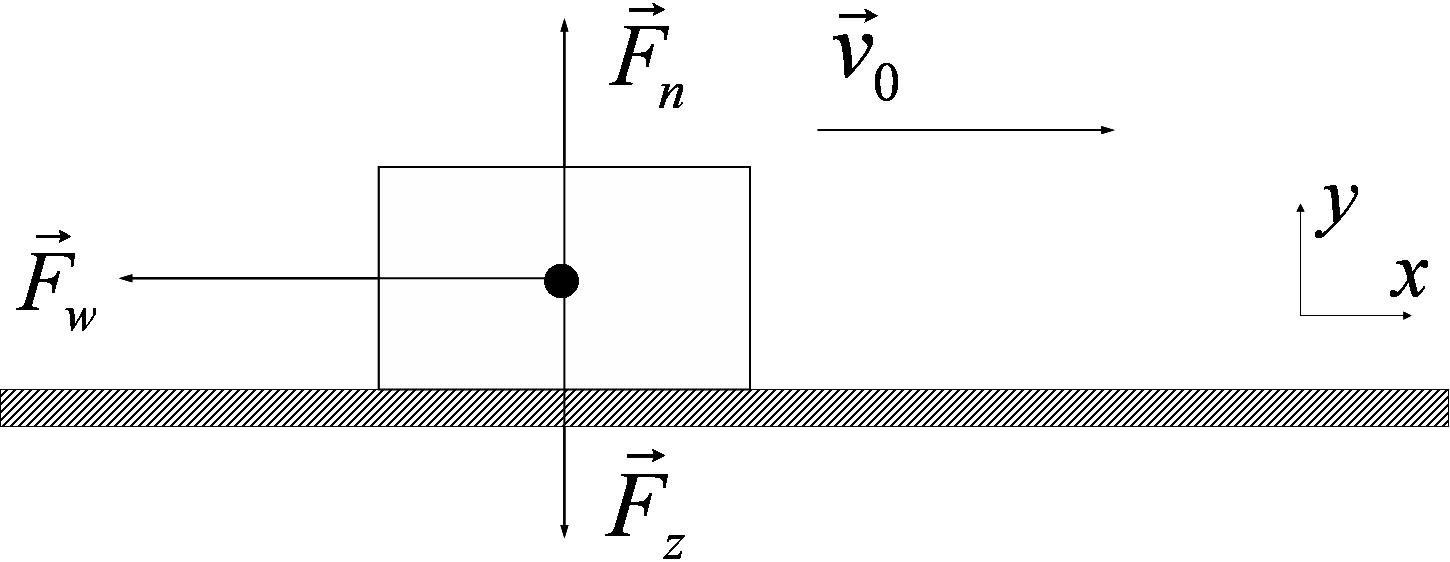
\includegraphics[width=0.5\textwidth ,angle=0]{hockeypuck2}
\end{center}
\end{figure}
\newline
\item [\textit{gegeven}]
\begin{tabular}[t]{lcl}
$v_0$ &$=$& $20,5~\rm m/s$\\
$x$ &$=$& $120~\rm m$\\
\end{tabular}
\item [\textit{gevraagd}]
$\mu$
\item [\textit{oplossing}]
De wrijvingskracht is de enige kracht volgens de horizontale
richting en vormt dus de resulterende kracht. Omdat ze tegengesteld
is aan de $x$-as geldt $F_{w,x}=-F_w$. Met $F_w=\mu F_n$ vinden we
voor de versnelling:
\begin{eqnarray}
-F_w &=& ma\nonumber\\
&\Downarrow& \nonumber\\
-\mu mg &=&ma\nonumber\\
&\Updownarrow& \nonumber\\
a &=& -\mu g\label{a}
\end{eqnarray}
De tijd uit de vergelijkingen voor een EVRB elimineren, waarbij de
eindsnelheid $v$ en de beginpositie $x_0$ nul zijn, levert:
\begin{eqnarray}
v&=&v_0+at\nonumber\\
x&=&x_0+v_0t+\frac{1}{2}at^2\nonumber\\
&\Downarrow&\nonumber\\
0&=&v_0+at\Leftrightarrow t=-\frac{v_0}{a}\nonumber\\
x&=&v_0\left(-\frac{v_0}{a}\right)+\frac{1}{2}a\left(-\frac{v_0}{a}\right)^2\nonumber\\
&\Downarrow&\nonumber\\
a&=&-\frac{v_0^2}{2x}\label{-v_0^2/2x}
\end{eqnarray}
Vergelijking (\ref{-v_0^2/2x}) samen met (\ref{a}) levert dan:
\begin{eqnarray}
\mu &=& \frac{v_0^2}{2gx}\label{remvgl}\\
&&\nonumber\\
&=& 0,178\nonumber
\end{eqnarray}
\end{oplossing}

\end{exercise}
 % hockeyschijf
% !TEX root = ../main.tex




\item\pt{5}\begin{minipage}[t]{.7\textwidth}
(\emph{Toestel van Atwood}) Twee verschillende massa's zijn via een katrol van te verwaarlozen massa met elkaar verbonden zoals in de figuur. De wrijving is eveneens te verwaarlozen. 
\newline
\newline
Bepaal de grootte van de versnelling van beide massa's en de spankracht in het touw.
\end{minipage}
\hfill
\begin{minipage}[t]{.2\textwidth}
\flushright
	\raisebox{1ex-\height}{%
		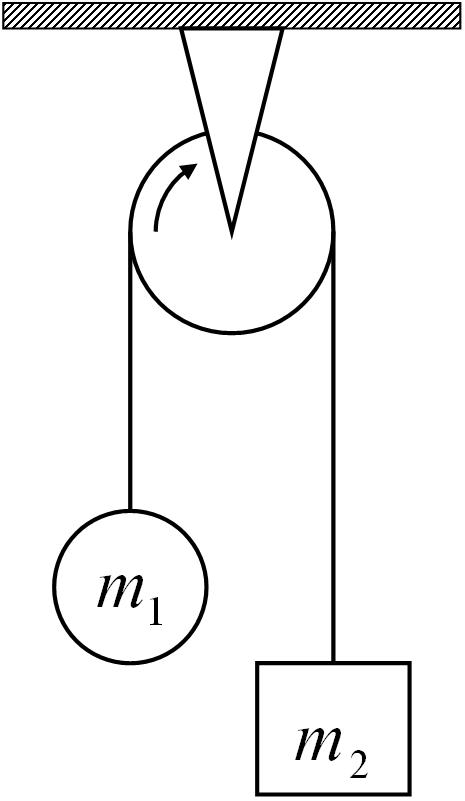
\includegraphics[height=4cm]{toestelatwood}
	}
\end{minipage}

\begin{oplossing}
$a=\frac{m_2-m_1}{m_1+m_2}g \quad F_s=\frac{2m_1m_2}{m_1+m_2}g$
\end{oplossing} % Toestel van Atwood

\begin{exercise}

 \begin{minipage}[t]{.62\linewidth}
Een massa blijft liggen op een draai\-tafel die met een hoeksnelheid van \SI{5,0}{rad/s} draait. Ze ligt op een afstand van \SI{10}{cm} van het middelpunt.
\newline
\newline
Hoe groot moet de wrijgvingsco\"effici\"ent tussen de massa en de tafel minstens zijn? Toon aan.
\end{minipage}
%\hspace{.05\linewidth}
\hfill
\begin{minipage}[t]{.33\linewidth}
	\raisebox{1ex-\height}{%
    	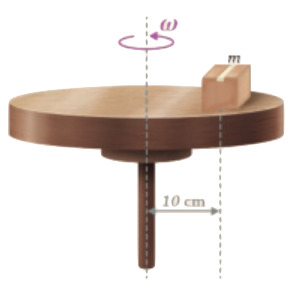
\includegraphics[width=\linewidth]{dyn/exercises/FV6p153}
  	}%
\end{minipage}

\begin{oplossing}
	De middelpuntzoekende kracht wordt door de wrijvingskracht geleverd. De maximale grootte hiervan wordt gegeven door $\mu F_n$. De hoeksnelheid die we nog net kunnen aanhouden zonder dat de massa's schuiven, vinden we met de tweede wet van Newton:
	\begin{eqnarray*}
		\vec{F}&=&m\vec{a}\\
		&\Downarrow&\\
		\mu mg&=&mr\omega^2
		%\Leftrightarrow\omega&=&\sqrt{\frac{\mu g}{r}}
	\end{eqnarray*}
	of
		\begin{eqnarray*}
\omega=\sqrt{\frac{\mu g}{r}}
	\end{eqnarray*}
Omdat de massa geen rol speelt in deze formule (voor een grotere massa is een grotere middelpuntzoekende kracht nodig maar de normaalkracht wordt evenredig groter voor grotere massa's), bepaalt de kleinste $\mu$ de maximale hoeksnelheid:
 \begin{eqnarray*}
\omega=\sqrt{\frac{\mu g}{r}}=6,52\rm\,rad/s
	\end{eqnarray*}
\end{oplossing}

\end{exercise}
 % FV 6 p. 153
%%TODO includes pdf ... %% 
\begin{exercise}

% !TEX root = ../main.tex



\pt{6}\begin{minipage}[t]{.6\linewidth}
	 De nevenstaande figuur toont een stel voorwerpen die met elkaar verbonden zijn met massaloze touwen die wrijvingsloos bewegen over katrollen. Het voorwerp met massa $2m$ schuift over een horizontale tafel. $m$ is gelijk aan \SI{2,0}{kg}. Alle voorwerpen hebben een versnelling van \SI{1,5}{m/s^2}. 
\end{minipage}
\hfill
\begin{minipage}[t]{.37\linewidth}
	\raisebox{1ex-\height}{%
		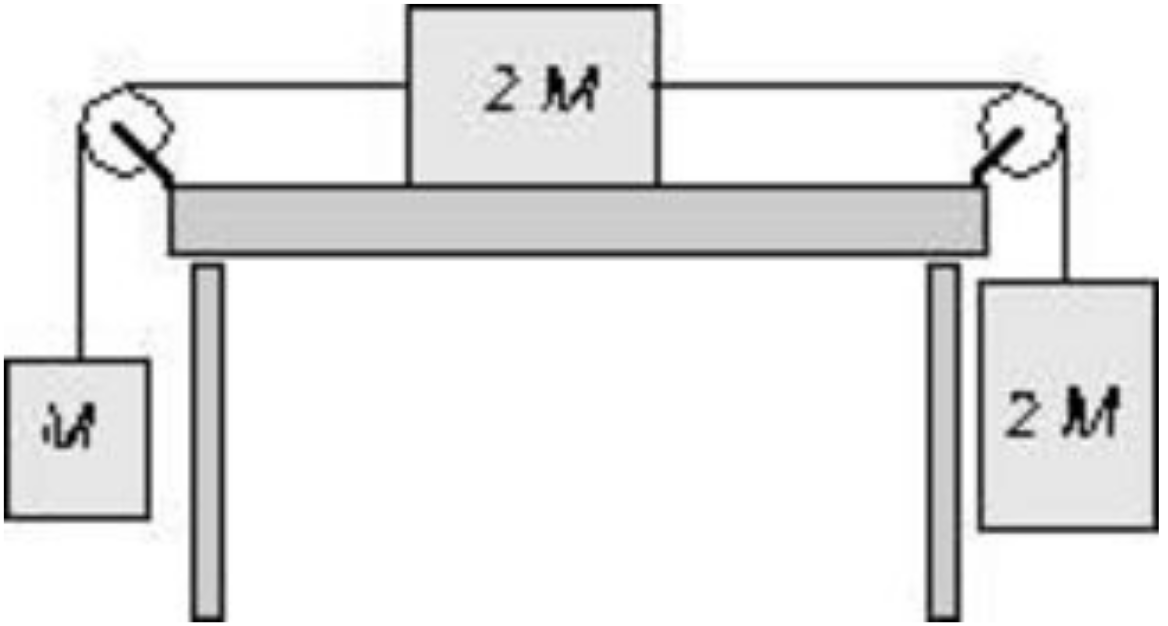
\includegraphics[width=\textwidth]{dyn/exercises/drieblokken_2}%
		} 
\end{minipage}

\begin{enumerate}
	\item Teken alle krachten op de blokken.
	\item Bepaal de grootte van de wrijvingskracht op het blok dat over de tafel glijdt.
\end{enumerate}



\begin{oplossing}
	\includepdf[pages={1},scale=.8]{./opl/VFO_9_8.pdf}
\end{oplossing}

\end{exercise}
 % Blokken op een tafel
% !TEX root = ../main.tex



\item\pt{1}Hoe kan een man die \SI{686}{N} weegt langs een touw naar beneden glijden, dat slechts \SI{600}{N} kan dragen zonder te breken?

Stel dat de man inschat dat hij, zonder zijn botten te breken, in staat is te springen van toch wel \SI{3,0}{m} hoog. Van hoe hoog zou hij dan met een dergelijk touw kunnen ontsnappen?



\begin{oplossing}
Door niet met zijn volle gewicht aan het touw te gaan hangen kan de man verhinderen dat het touw breekt. Het gevolg is wel dat hij een nettokracht naar beneden ondervindt waardoor hij toch naar beneden versnelt, al is het met een kleinere versnelling dan de valversnelling.

Door met \SI{600}{N} aan het touw te trekken, ondervindt hij een spankracht omhoog met diezelfde grootte. Met een referentieas naar beneden volgt uit $F_z-F_s=ma$ en uit $m=\frac{F_z}{g}$ voor de versnelling van de man:
\begin{equation}
	a=\left(1-\frac{F_s}{F_z}\right)g\label{versnelling_ontsnapper}
\end{equation}
wat gelijk is aan \SI{1,23}{m/s^2}.

Uit $v^2=v_0^2+2ax$ volgt de maximale snelheid die hij bij de impact op de grond aankan als we voor $a$ de valversnelling $g$ nemen en voor $x$ de gegeven \SI{3,0}{m}. Uit diezelfde formule vinden we de hoogte $h$ vanwaar de man kan ontsnappen als we nu de netto versnelling $a=\SI{1,23}{m/s^2}$ (\ref{versnelling_ontsnapper}) nemen: 
\begin{equation*}
	h=\frac{v^2}{2a}=\ldots=\frac{F_z}{F_z-F_s}x
\end{equation*}
wat gelijk is aan \SI{24}{m}.
\end{oplossing} % Ontsnappen langs een touw

\begin{exercise}

% !TEX root = ../main.tex



 Drie voorwerpen zijn aan elkaar verbonden met touwtjes. De wrij\-vings\-factor tussen de tafel en het erop liggend voorwerp $V$ is $\mu$.
\begin{figure}[h]
\begin{center}
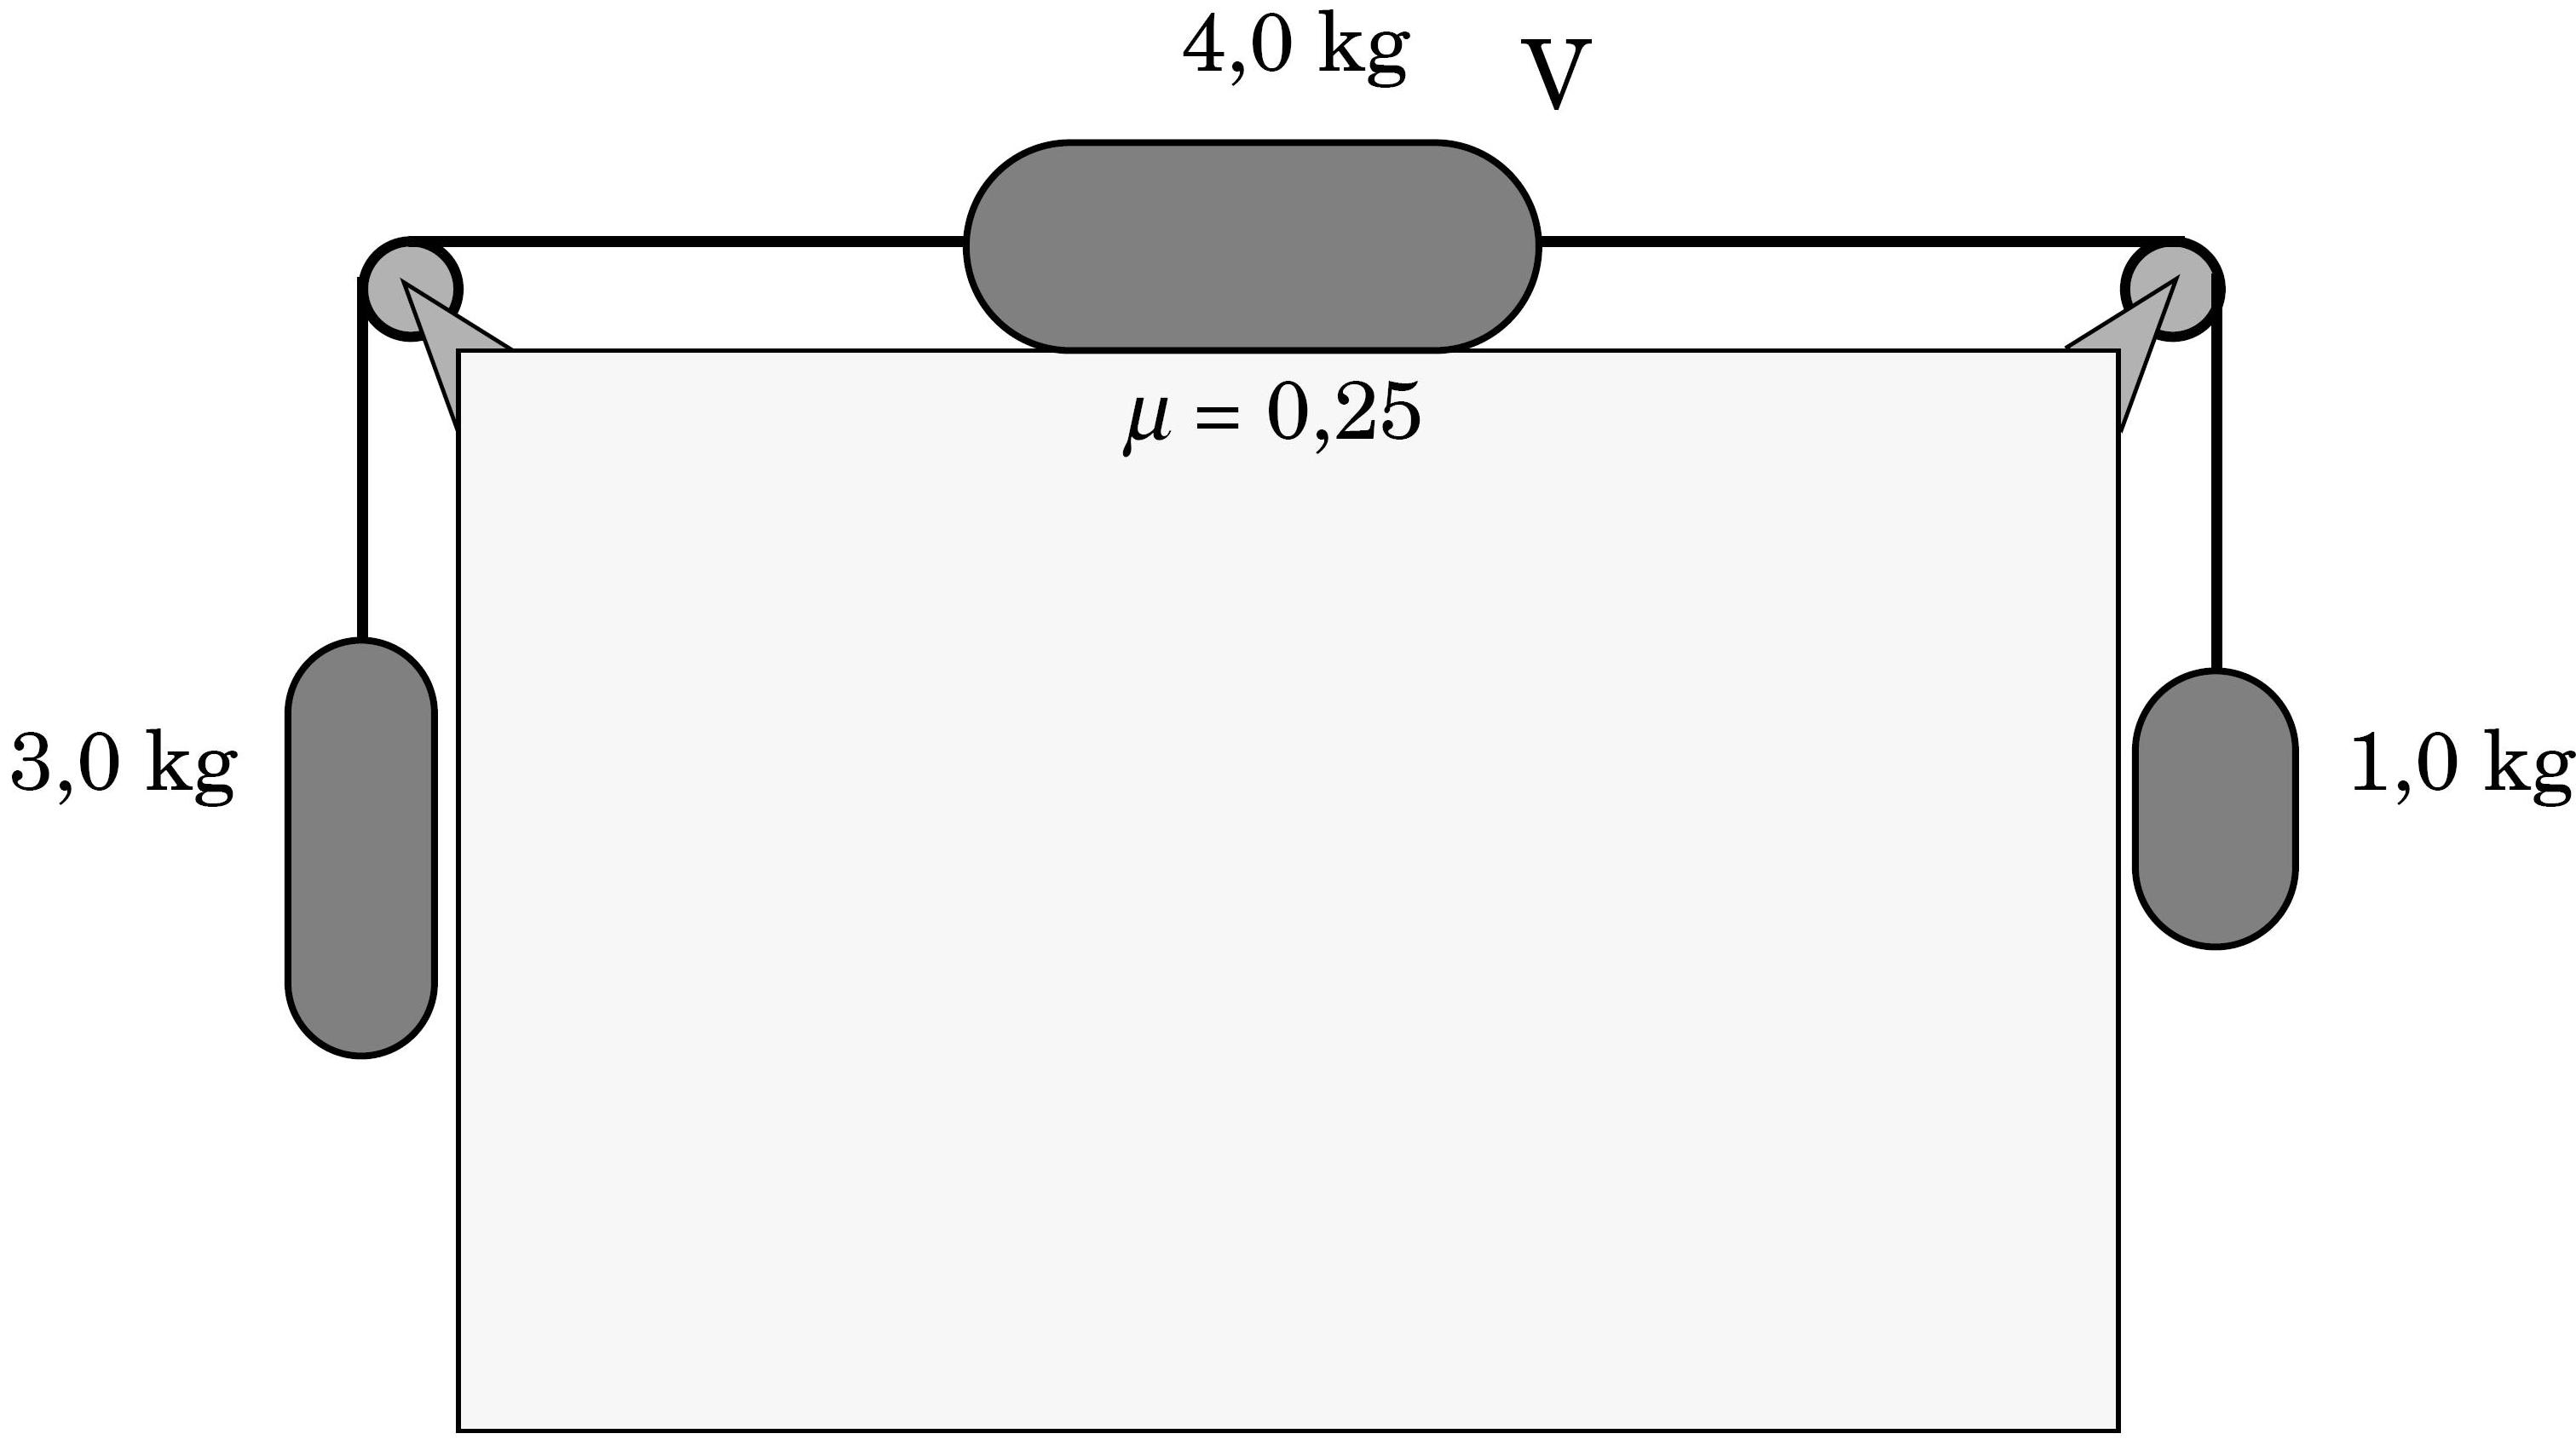
\includegraphics[width=0.6\textwidth ,angle=0]{drie_voorwerpen}
\end{center}
\end{figure}
Veronderstel dat er geen wrijving is in de katrollen en dat de massa van de katrollen te verwaarlozen is. Bepaal de versnelling van het voorwerp. (Bron: 16de VFO 2004)
\begin{oplossing}
\newline
Om de versnelling van het voorwerp te vinden kunnen we de tweede wet van Newton toepassen op de drie massa's. We tekenen de krachtendiagrammen op elk van de massa's (zie figuur). 
\begin{figure}[h]
\begin{center}
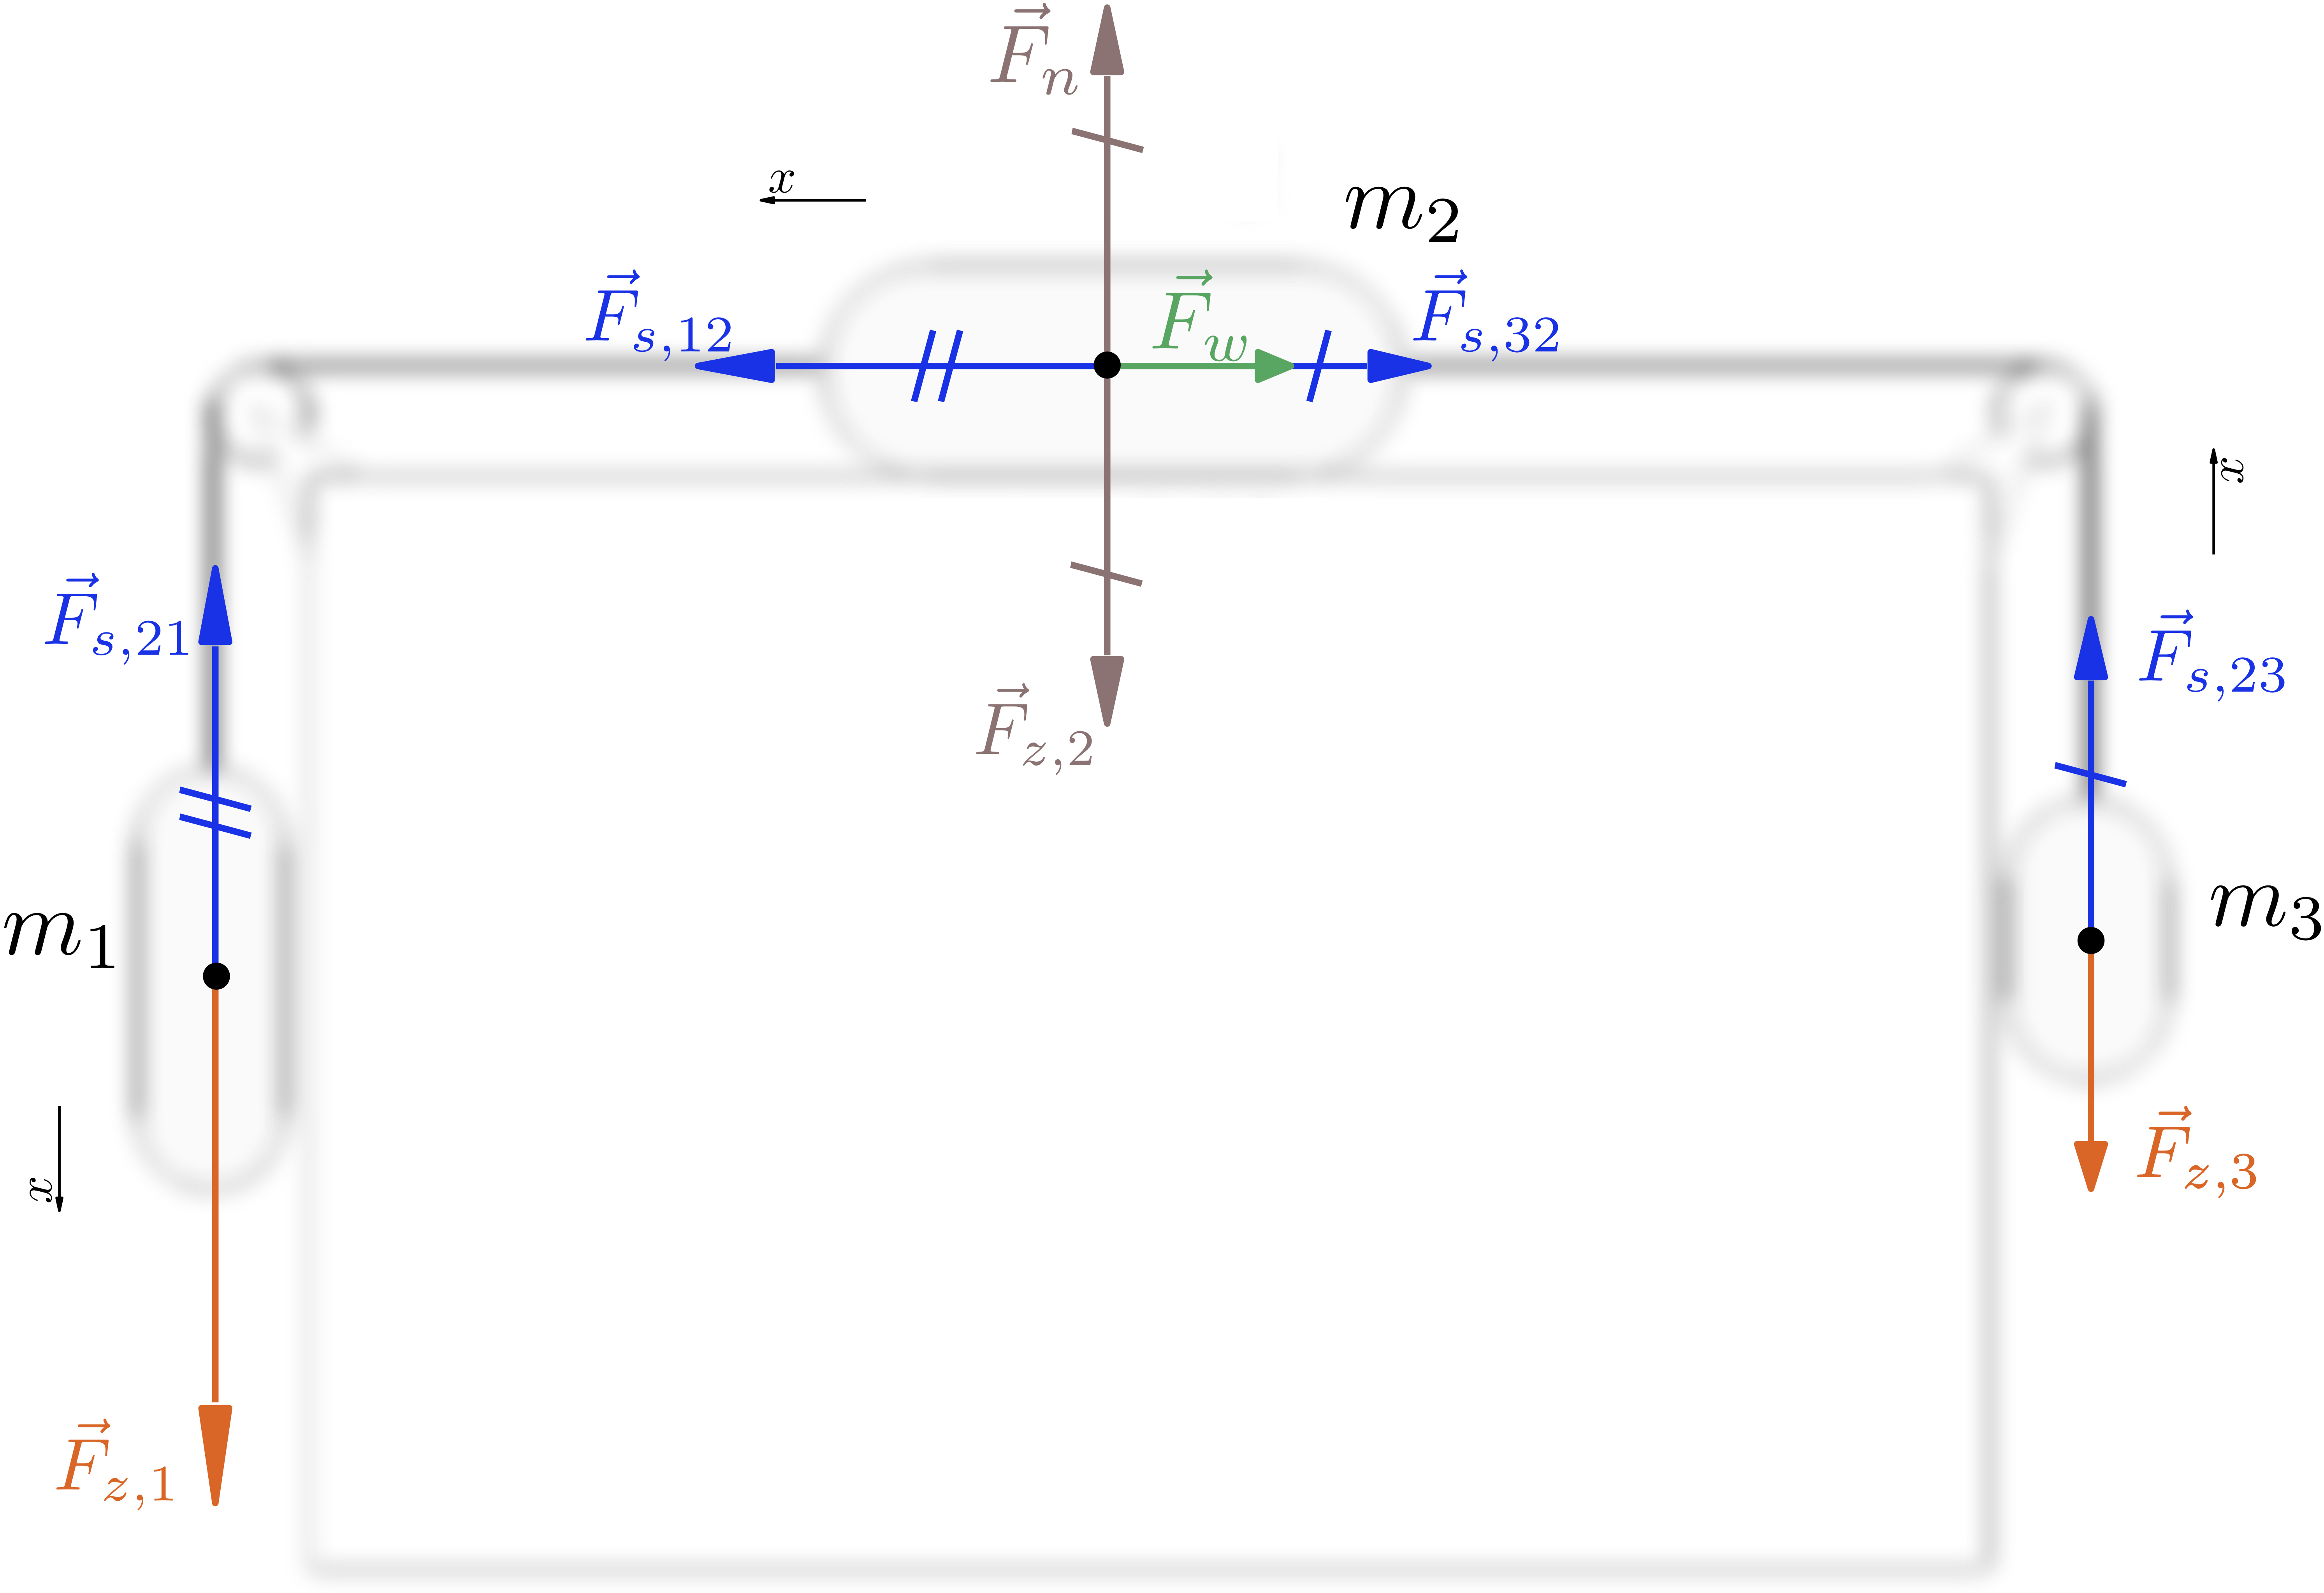
\includegraphics[width=0.73\textwidth ,angle=0]{drie_voorwerpen_krachten}
\end{center}
\end{figure}
\newline
Voor $m_1$ vinden we, met de keuze van de $x$-as verticaal naar beneden:
\begin{eqnarray}
F_{z,1}-F_{s,21}=m_1a\label{m_1}
\end{eqnarray}
Voor $m_3$ vinden we, met nu de keuze van de $x$-as verticaal naar boven:
\begin{eqnarray}
F_{s,23}-F_{z,3}=m_3a\label{m_3}
\end{eqnarray}
Voor $m_2$ vinden we, met de keuze van de $x$-as horizontaal naar links:
\begin{eqnarray}
F_{s,12}-F_w-F_{s,32}=m_2a\label{m_2}
\end{eqnarray}
Volgens de derde wet van Newton kunnen we de overeenkomstige spankrachten aan mekaar gelijk stellen: $F_{s,21}=F_{s,12}$ en $F_{s,32}=F_{s,23}$. Samen met $F_w=\mu F_n$ en $F_z=ma$ hebben we drie vergelijkingen en drie onbekenden. Oplossen naar de versnelling levert:
\begin{eqnarray*}
a=\frac{m_1-m_2-\mu m_3}{m_1+m_2+m_3}g=1,2\rm\,m/s^2
\end{eqnarray*}
\newline
\newline
Realiseer je dat de keuze van de $x$-as bij het bepalen van de componenten van de krachten de tekens bepalen van die componenten -- en ook die van de versnelling. Als je bijvoorbeeld tweemaal $a$ schrijft (in vergelijking (\ref{m_1}) en (\ref{m_3})) moet het ook effectief over dezelfde versnelling gaan, en niet over versnellingen die elkaars tegengestelde zijn. Met de $x$-as verticaal naar beneden geori\"enteerd voor $m_1$, zal de versnelling voor $m_1$ positief zijn als de massa naar beneden versnelt (wat hij doet; $m_1>m_3$). Voor $m_3$ moet je dan de $x$-as verticaal omhoog kiezen, wil je dat $a$ evenzeer positief is of dus dezelfde betekenis heeft.
\newline
\newline
Zie ook dat uit vergelijking (\ref{m_1}) volgt dat $m_1$ niet met de zwaartekracht aan $m_2$ trekt! De massa $m_1$ versnelt, waarvoor een resulterende kracht nodig is. 
\end{oplossing}

\end{exercise}
 % Drie voorwerpen 16de VFO 2004
% !TEX root = ../main.tex



\item \begin{minipage}[t]{.67\linewidth}
Een munt met een massa van \SI{3,0}{g} ligt op een blokje van \SI{20,0}{g}. Het geheel ligt op een draaiende schijf op \SI{12,0}{cm} van de rotatieas. Als de wrijvingsco\"effici\"ent tussen de munt en het blokje 0,52 is, en de wrij\-vings\-co\"effici\"ent tussen het blokje en de schijf 0,75 is, welke hoeksnelheid mag de schijf dan maximaal hebben zodat noch de munt noch het blokje wegschuift?
\end{minipage}
\hfill
\begin{minipage}[t]{.3\linewidth}
	\raisebox{1ex-\height}{%
    	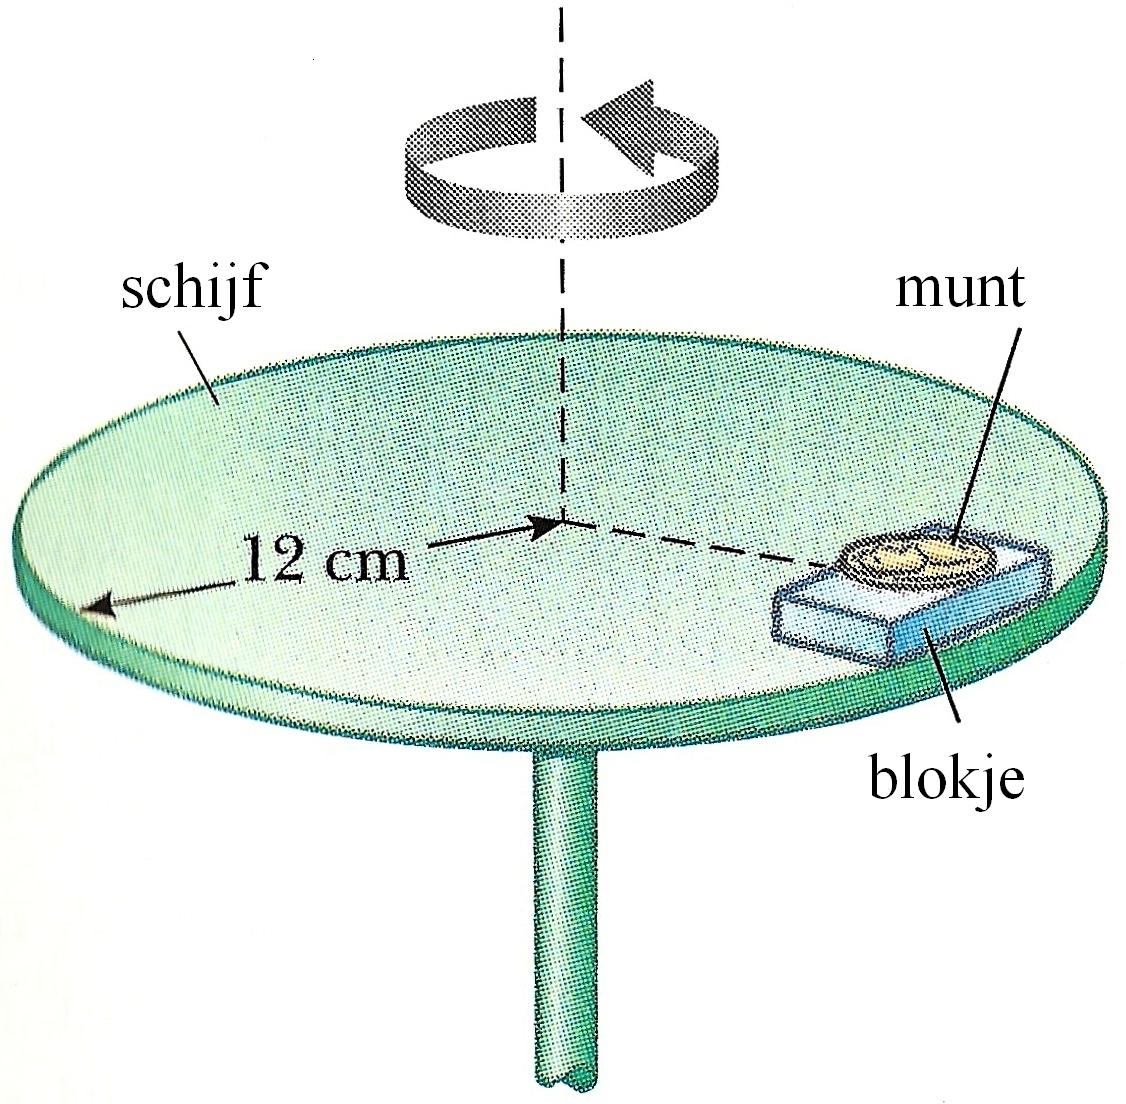
\includegraphics[width=\linewidth]{muntblokjeopschijf}%
  	}%
\end{minipage}

\begin{oplossing}
	De middelpuntzoekende kracht die nodig is om de objecten te laten ronddraaien, wordt door de wrijvingskracht geleverd. De maximale grootte hiervan wordt gegeven door $\mu F_n$. De hoeksnelheid die we nog net kunnen aanhouden zonder dat de massa's schuiven, vinden we met de tweede wet van Newton, $\vec{F}=m\vec{a}$:
	\begin{eqnarray*}
%		\vec{F}&=&m\vec{a}\\
%		&\Downarrow&\\
		\mu mg&=&mr\omega^2
		%\Leftrightarrow\omega&=&\sqrt{\frac{\mu g}{r}}
	\end{eqnarray*}
	of
		\begin{eqnarray*}
\omega=\sqrt{\frac{\mu g}{r}}
	\end{eqnarray*}
	
Hierin hebben we gebruikt dat de massa's in de verticale richting niet versnellen en dus de normaalkracht op de massa's even groot is als de zwaartekracht op die massa's. Ook hebben we gebruikt dat de versnelling van een object dat een eenparig cirkelvormige beweging uitvoert, gegeven wordt door $a=r\omega^2$.

Omdat de massa geen rol\footnote{De massa speelt geen rol omdat hij niet in de formule voorkomt. Dat is een hard wiskundig argument. Een kwalitatieve uitleg is dat voor een grotere massa weliswaar een grotere middelpuntzoekende kracht nodig is maar dat de normaalkracht ook evenredig groter wordt met de massa, en dus ook de wrijvingskracht.} speelt in deze formule, bepaalt de kleinste $\mu$ de maximale hoeksnelheid:
 \begin{eqnarray*}
\omega=\sqrt{\frac{\mu g}{r}}=\SI{6,52}{rad/s}
	\end{eqnarray*}
\end{oplossing} % munt en blokje op een draaiende schijf

\begin{exercise}

% !TEX root = ../main.tex



 Een steen wordt aan een touwtje rondgeslingerd met een snelheid die in grootte constant is. 

\begin{enumerate}
	\item\pt{2}Heeft de steen een versnelling?
	\item\pt{2}Ondervindt de steen een resulterende kracht?
\end{enumerate}

Leg uit.

\end{exercise}
 % Steen aan een touwtje

\begin{exercise}

 
\begin{minipage}[t]{0.5\textwidth}
Welke snelheid moet een achtbaanwagentje dat op zijn kop boven in een lus aankomt ten minste hebben, willen de passagiers niet naar beneden vallen? Neem aan dat de kromtestraal van de lus $7,0\rm\,m$ bedraagt.
\end{minipage}
\hspace{5mm}
\begin{minipage}[t]{0.45\textwidth}
\raisebox{-2cm}{
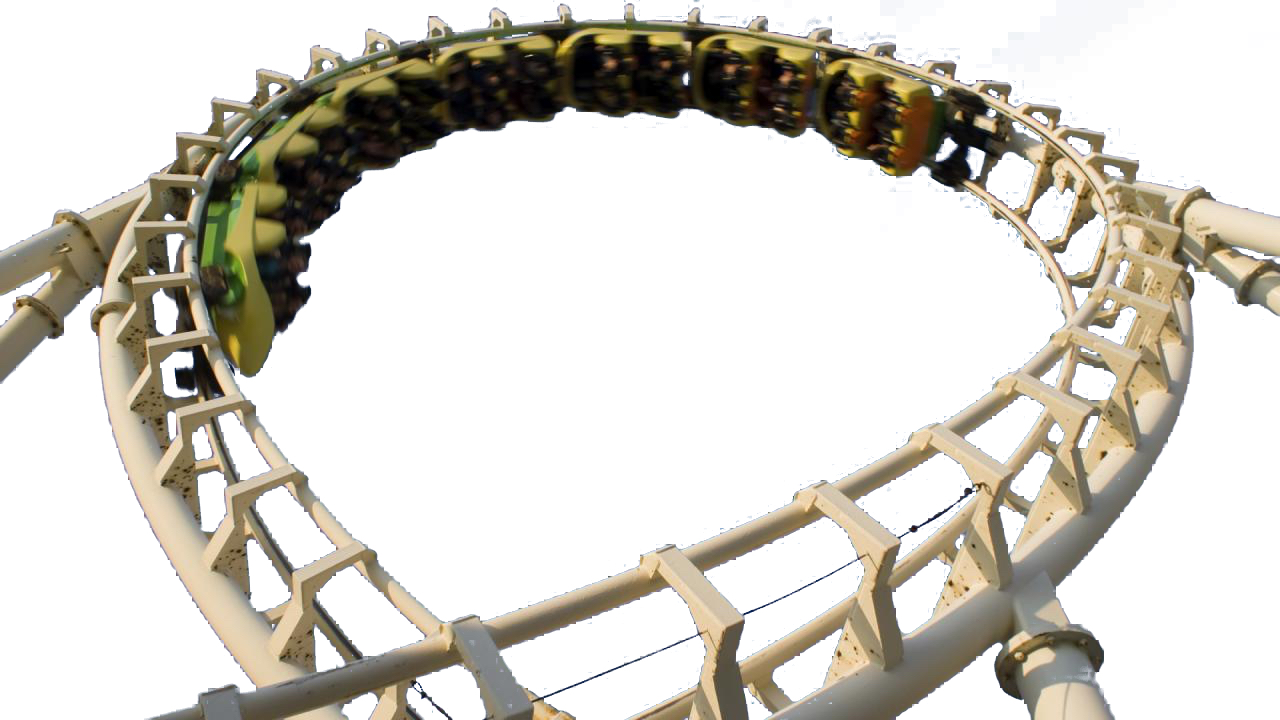
\includegraphics[width=0.9\textwidth]{dyn/exercises/gewonden-ontsporing-achtbaan-vs_res}
}
\end{minipage}
\begin{oplossing}
De snelheid moet groot genoeg zijn zodat de zwaartekracht er niet in slaagt de passagiers sneller uit de bocht te trekken dan noodzakelijk. Hoe trager de passagiers gaan, hoe minder groot de middelpuntzoekende kracht moet zijn om die beweging tot stand te brengen. 
\newline
Bij een snelheid die groot genoeg is, helpt de normaalkracht (door de wagentjes op de passagiers uitgeoefend) de zwaartekracht om een middelpuntzoekende kracht te genereren. De minimale snelheid vinden we dan ook wanneer de normaalkracht wegvalt en enkel de zwaartekracht de middelpuntzoekende kracht levert:
\begin{eqnarray*}
		F=ma\Rightarrow mg=\frac{mv^2}{r}
\end{eqnarray*}
Zodat:
$v_{\rm min}=\sqrt{rg}=8,29\rm\,m/s=29,8\rm\,km/h$.
\end{oplossing}

\end{exercise}
 % Looping 

\begin{exercise}

% !TEX root = ../main.tex



 Welk lichaam is verantwoordelijk voor de middelpuntzoekende kracht in de onderstaande gevallen. Noem tevens waar het mogelijk
is, de naam van de kracht die de middelpuntzoekende kracht levert bij:
\begin{enumerate}
\item de modder op de buitenomtrek van een draaiend fietswiel;
\item een trein die een bocht neemt;
\item een auto die een bocht neemt bij een horizontaal wegdek;
\item het ronddraaien in een horizontaal vlak van een steen aan een touw;
\item de verandering van de stroomrichting van het water in een bocht van een rivier;
\item een persoon in een ronddraaiende ton waarvan de bodem weggezakt is;
\item de beweging van de maan op haar baan rond de aarde;
\item de beweging van de elektronen rond de kern in een atoom
\end{enumerate}

\end{exercise}



%\import{./lib/}{dyn_ECB_II_1} % massa aan een touw in een auto in de bocht = verloren gegaan ...


\end{document}